\documentclass[12pt]{article}
\usepackage{verbatim}
\usepackage[dvips]{epsfig}
\usepackage{color}
\usepackage{url}
\usepackage[colorlinks=true]{hyperref}
\usepackage{enumitem} % [noitemsep,nolistsep] compact itemize/enumerate etc.
\usepackage[margin=2cm]{geometry}

% Typeface
\usepackage[condensed,math]{iwona}
\usepackage[T1]{fontenc}

\begin{document}

\section*{HETERARCH: Technical}

{\bf Related Documentation:}
% start: userdocs-tag-replace-items related-do-nothing
% end: userdocs-tag-replace-items related-do-nothing

\section*{Developer Content Management}

This document provides information for the {\bf \small Heterarch} Content Management System ({\bf \small HCMS}), an open source software platform that supports distributed personalized digital content broadcasting. It is developed and maintained by {\bf Neurospaces\,Development} in collaboration with {\bf Three\,Way\,Street}.

\subsection*{Interaction with HCMS Functionality}

{\bf \small HCMS} is accessed or controlled in one of three ways. This is determined by level of experience and the functionality required (see Definitions in \href{../heterarch-overview/heterarch-overview.tex}{\bf Heterarch\,Overview} for details):

\begin{enumerate}[noitemsep,nolistsep]
\item{\bf Browser Interface:} The user level interface. It allows users to interact with {\bf \small HCMS} content.
\item {\bf The Content Framework Graphic User Interface (CF-GUI):} The preferred developer interface. The commands the {\bf \small CF-GUI} implements are a subset of those available from the command line interface. It is accessible by repository owners and other authorized content developers and developers authorized by repository owners.
\item {\bf Command Line Interface:} All {\bf \small HCMS} functionality can be accessed and controlled from a command line prompt in a terminal window. It is the legacy developer level interface.
\end{enumerate}

\subsection*{Content Framework Graphic User Interface}

To simplify content management, a Graphic User Interface (GUI) is available.\\
The preferred {\bf \small Heterarch} Developer GUI is called the Content Framework Graphic User Interface ({\small \bf CF-GUI}).\\
\noindent It can be started from a (X-Window) command line prompt with the following command:

\begin{verbatim}
   heterarch-gui
\end{verbatim}

\noindent The {\small \bf CF-GUI} is the primary management tool for a {\bf \small HCMS} repository. The figure below illustrates the default appearance of this GUI.

\begin{figure}[h]
   \centering
   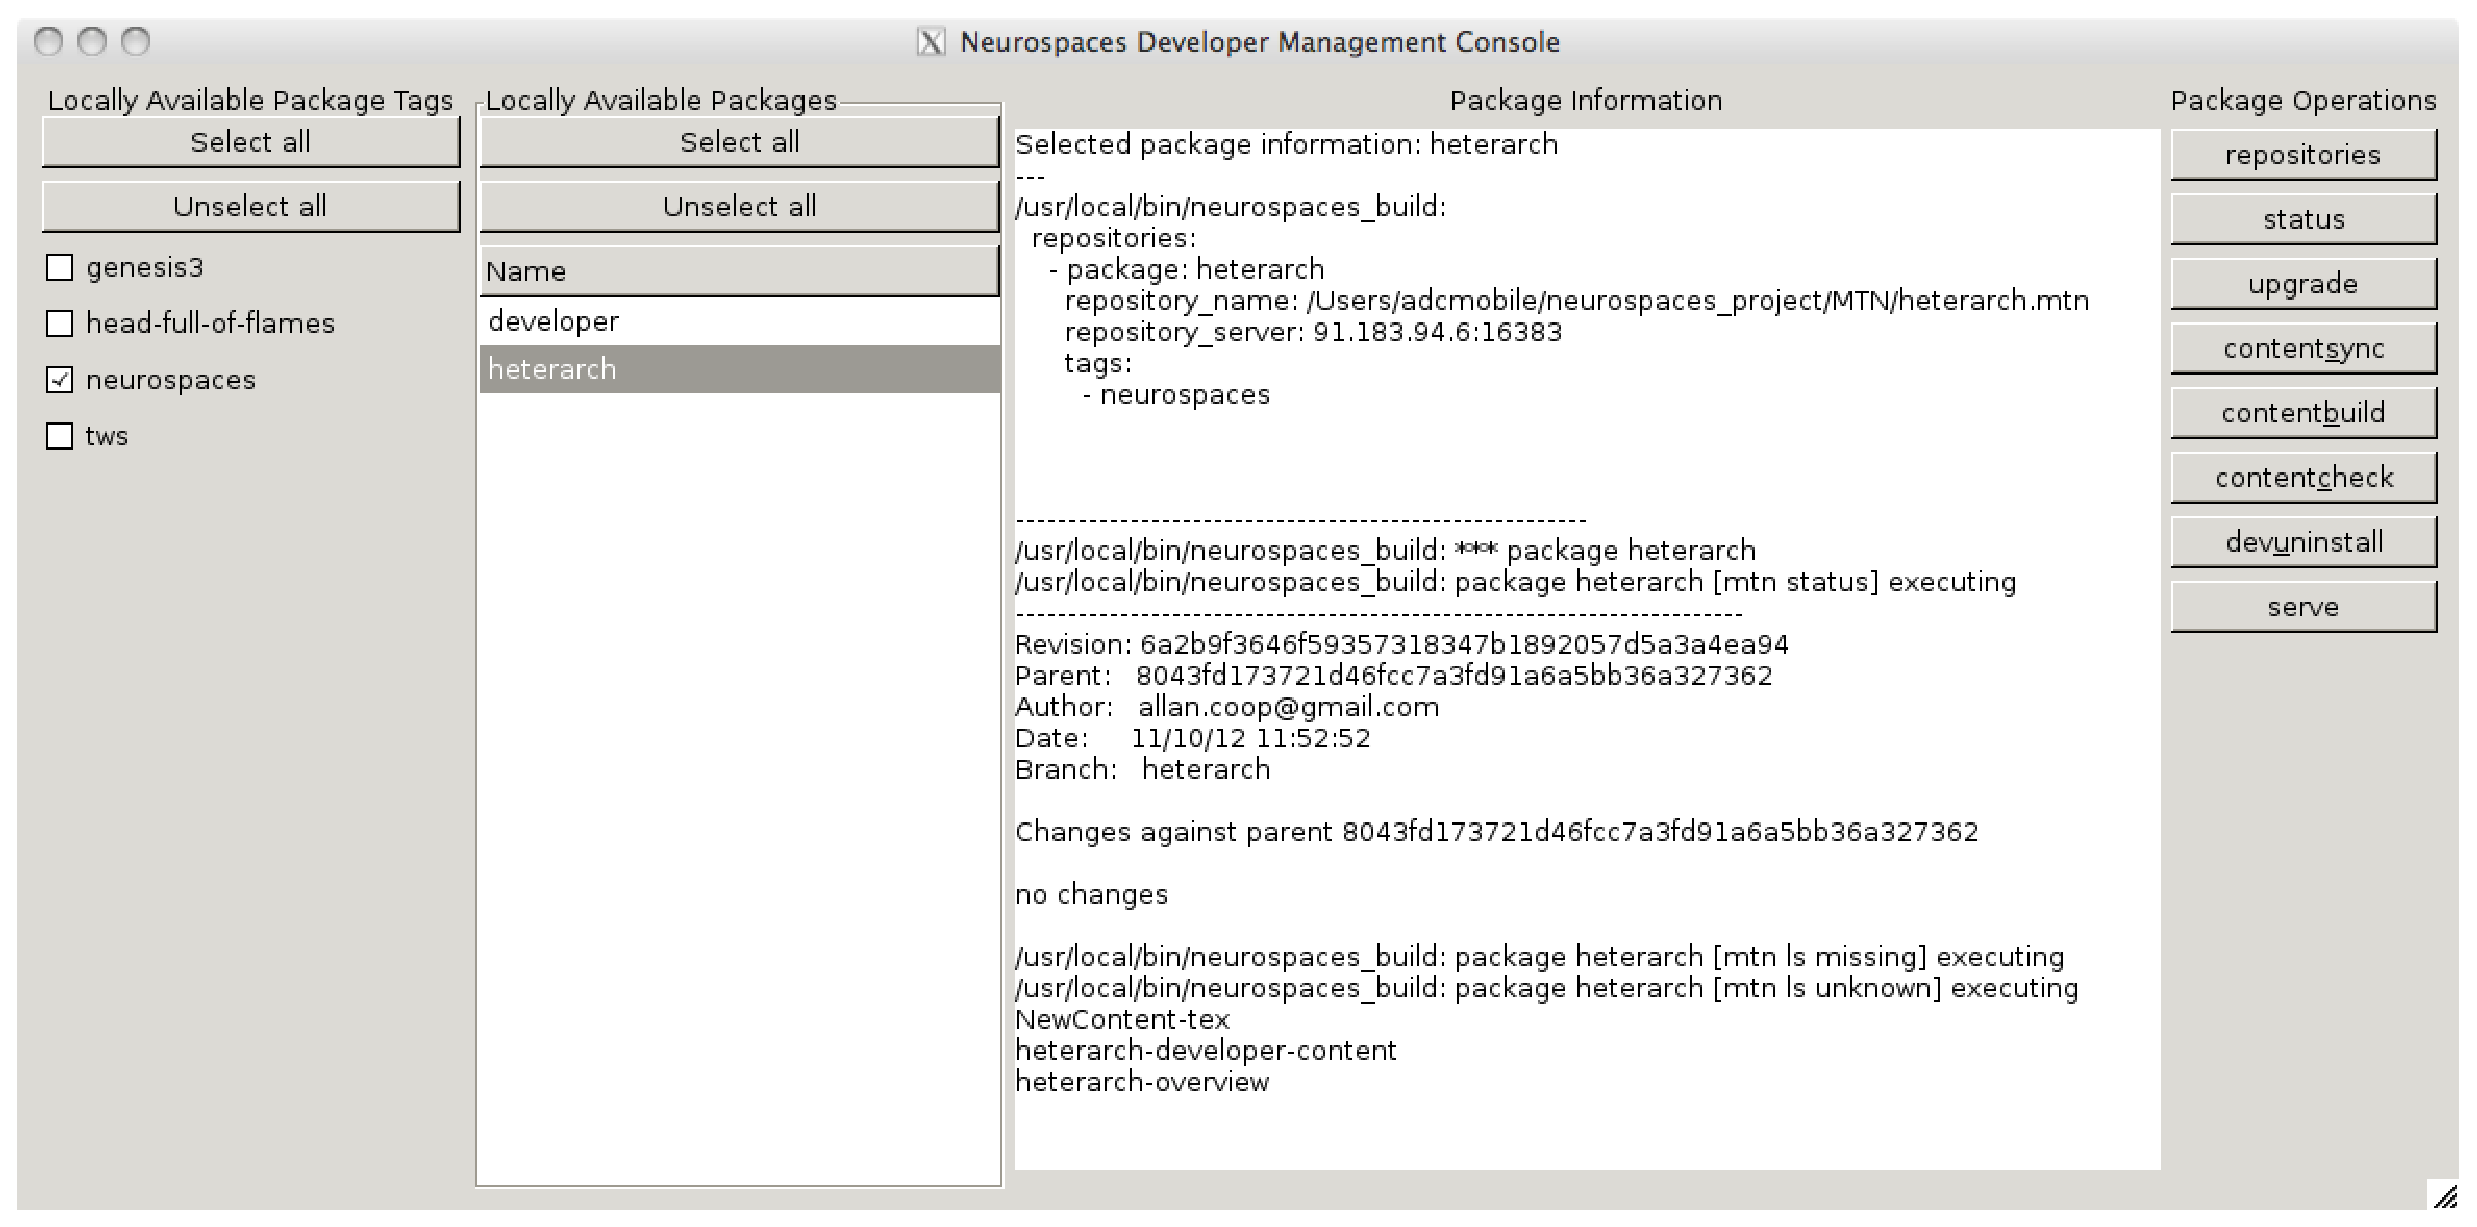
\includegraphics[scale=0.4]{figures/heterarch-developer-content-gui.eps}
\end{figure}

\subsection*{CF-GUI Components}

There are four functionally different panes arranged as columns in the {\small \bf CF-GUI}. From left to right they include: Locally Available Package Tags, Locally Available Packages, Package Information, and Package Operations.
We now introduce these different components.

\begin{enumerate}
\item {\bf Package Domains}\\
Tags listed under the {\bf \small Locally\,Available\,Package\,Tags} heading give the locally available package domains known to {\bf \small Heterarch}.\\
\noindent Selecting the check-box to the left of a given package domain tag generates a list of packages associated with the selected domain in the {\bf \small Locally\,Available\,Packages} window.

\item {\bf Available Packages}\\
The {\bf \small Locally\,Available\,Packages} pane lists all accessible packages within (check-box) selected package domains. Selecting an available package generates a listing of information about the package in the  {\bf \small Package\,Information} pane.

\item {\bf Package Information}\\
The {\bf \small Package\,Information} pane gives information about the location, status, and contents of the selected package. The listing is obtained through the version control functionality of {\bf \small HCMS}.  It includes:

\begin{description}[noitemsep,nolistsep] 
\item {\bf Repository name:} In the {\small \bf CF-GUI} example given above this is {\bf \small heterarch}.
\item {\bf Location of the package build script generating the report:} For the given example, {\tt \small /usr/local/bin/neurospaces\_build}.
\item {\bf Repository information known to version control:} Includes package and repository name, IP number of the server where the repository is located, and the repository tags.
\item {\bf Version control summary:} Includes content revision ID number and revision parent ID number. The name of the authorized content developer, date and time content item changes were put under version control, and the repository branch where any revised content will be maintained.
\item {\bf Content changes:} The content items accessed and altered in
  the {\small \bf workspace} are listed.
\item {\bf Missing files:} Any files found to be missing from the
  {\small \bf repository} are listed. (In the example given above, no
  files were found to be missing.)
\item {\bf Unknown files:} Any files in the {\small \bf workspace} but
  not under version control in the repository are listed.
\end{description}

\subsubsection*{Package Operations}

Buttons listed under this heading provide the following {\bf \small HCMS} functionality:

\begin{description}[noitemsep,nolistsep] 
\item {\bf repositories}\\
Run operation {\tt \small neurospaces\_repository}.
\item {\bf status}\\
Run operation {\tt \small neurospaces\_status}.
\item {\bf upgrade}\\
Run operation {\tt \small neurospaces\_upgrade}.
%\item {\bf pull}\\
%Run operation {\tt \small neurospaces\_pull}.
%\item {\bf sync}\\
%Run operation {\tt \small neurospaces\_sync}.
\item {\bf content\underline{s}ync}\\
Run operation {\tt \small neurospaces\_content\_sync}.
\item {\bf clean}\\
%Run operation {\tt \small neurospaces\_clean}.
%\item {\bf update}\\
%Run operation {\tt \small neurospaces\_update}.
%\item {\bf diff}\\
%Run operation {\tt \small neurospaces\_diff}.
%\item {\bf configure}\\
%Run operation {\tt \small neurospaces\_configure}.
%\item {\bf install}\\
%Run operation {\tt \small neurospaces\_install}.
%\item {\bf check}\\
%Run operation {\tt \small neurospaces\_check}.
\item {\bf content\underline{b}uild}\\
Run operation {\tt \small neurospaces\_content\_build}.
\item {\bf content\underline{c}heck}\\
Run operation {\tt \small neurospaces\_content\_check}.
\item {\bf dev\underline{u}ninstall}\\
Run operation {\tt \small neurospaces\_dev\_\underline{u}ninstall}.
\item {\bf serve}\\
Run operation {\tt \small neurospaces\_serve}.
\end{description}

\end{enumerate}

\subsection*{Manually Create New Repository}

To manually create a new repository on your local machine the following steps must be completed. 

\begin{enumerate}[noitemsep,nolistsep]
\item Contact {\bf \small Three\,Way\,Street} with the name of your new repository. In return you will receive a new build configuration. It should be added to your local configuration file located at:\\
  \hspace*{5mm}{\tt /etc/neurospaces/developer/build.yml}
  
You can check the status of this file with the following command entered at a command line prompt in a terminal window:
\begin{verbatim}
   neurospaces_packages
\end{verbatim}
It should list the name of the new package and confirms that addition of the new build configuration to the {\tt \small build.yml} configuration file was successful:
\begin{verbatim}
---
enabled packages in order of build:
    - developer
    - heterarch
    - tws
    - occupy
    - cough-cough
    - head-full-of-flames
    - overflow-design
\end{verbatim}
Note: As it is a yml file, the {\tt \small build.yml} file is white space sensitive.

  \marginpar{we should fold this in into the {\bf \small
      Configurator}, a package that has been under design for 7 years
    or so, now seems the right time to implement it.}
\item {\bf On all machines of interested clients:} After updating your local {\tt \small build.yml} configuration file as described above, the following commands should  be run in the given order at a command line prompt  in a terminal window.\\
(Note: You should replace $<$repository-name$>$ with the name of the repository you want to build. To simplify naming, we recommend you follow the {\bf \small HCMS} naming convention which is to replace white space with a single dash (-)):
\begin{verbatim}
   neurospaces_create_directories <repository-name>
   neurospaces_pull <repository-name>
   neurospaces_update <repository-name>
   neurospaces_configure <repository-name>
   neurospaces_install <repository-name>
\end{verbatim}
\item If you make a mistake you can remove what you have done by running the following commands:
\begin{verbatim}
   cd ~/neurospaces_project/<repository-name>
   rm -fr source/snapshots/0
   cd ~/neurospaces\_project
   rm MTN/<name>.mtn
\end{verbatim}

\item {\bf Check write access where necessary:} After completion of repository installation steps, the following command should  be run at a command line prompt  in a terminal window to confirm that all write accesses are correctly configured.

\begin{verbatim}
   neurospaces_sync <repository-name>
\end{verbatim}

\item {\bf Check integration with the developer package:} Make sure {\tt \small sudo}\marginpar{needs documentation, should be working anyway in the virtual machine that we will configure} is working, then issue the following commands from the prompt in a terminal window:

\begin{verbatim}
   neurospaces_update <repository-name>
   neurospaces_configure <repository-name>
   neurospaces_install <repository-name>
\end{verbatim}
\end{enumerate}

\subsection*{Manual Content Creation}

The command to create a new content item may be issued manually at a command line prompt when it is located within the repository where the item is to be created.

{\bf There must be only one content item located in each in each content item folder/directory.}

The content item name should follow the {\bf \small HCMS} content-naming convention--words in the name are separated by a single dash--where {\tt <\dots>} is replaced with the unique name. The command takes the following:
\begin{verbatim}
   <repository-name>-create <content-name>
\end{verbatim}

This command automatically generates the unique content management structure required to support a given content item. The structure is obtained from a built-in content item template called {\it NewDocument} which is automatically placed in a repository when it is created.

\subsubsection*{NewDocument Template}

The {\it NewDocument} directory/folder provides a template for the creation of a new text-based content item.\\
{\bf Importantly}, the name of this directory/folder and its contents should not be changed.\\
By default, {\it NewDocument} contains two relevant files and a directory, as well as any other {\bf \small} files or directories required to locally manage the content item within the repository:

\begin{description}[noitemsep,nolistsep] 
	\item {\tt descriptor.yml}\\
	The name of the descriptor file\,{\it descriptor.yml} should never be changed. The default contents of this file include: attributes (terminated by a colon) and tags (indicated by a hyphen).
	\item {\tt NewDocument.tex}\\
	The default content creation editor for {\bf \small HCMS} is \LaTeXe. If you want to use a different editor, at any time prior to content creation, the default may be changed to your preferred format by replacing the NewDocument file with a file in a format of your choice and recognized by the {\bf \small HCMS}. These include: OpenOffice ({\tt odf}--the preferred default format), MS Word ({\tt doc}), Rich Text Format ({\tt rtf}), and Structured Text Format ({\tt rst}).
	\item {\tt figures}\\
	The name of the {\it figures} directory should never be changed. Figures to be included in a content item are located in this directory/folder. The format of these files will be determined by the requirements of the content item file format you choose. For \LaTeXe, the {\it figures} format is Encapsulated Postscript ({\tt eps}).
\end{description}

\subsubsection*{Descriptor File}

Individual content items are maintained in association with a unique human readable, YAML-based file named {\it descriptor.yml}. This file is white space sensitive and contains four attribute lines (indicated by a colon ``:''). The first three {\it descriptorfile.yml} attributes are self explanatory and include, (i) a comment line, (ii) one line description of the associated content item (both indicated by: {\small{$<\ldots>$}}), (iii) and the name of the given content item in the repository (automatically inserted into the descriptor file when it is generated during content item creation). The fourth attribute is divided into two types of ``tag'' (indicated by a hyphen ``-''  and {\small{$<<\ldots>>$}}).

The two types of tag recognized by {\bf \small HCMS} include, (i) control tags that define relationships between content items, and their type and visibility, and (ii) automatically generated data tags which define data flows independently of any internal hyperlinking between content items. These tags can be used to organize content items and create, for example, reader flows.

The default form of the descriptor file is:
\begin{verbatim}
---
comment: <Optional comment.>
description: <One line description of content item.>
document name: content-name
tags:
  - <identifier--order number>
  - <domain--order number>
  - <format>
  - <visibility>
\end{verbatim}
Angle braces (e.g. {\small{$<\ldots>$}}) should be manually replaced as described above.
\begin{description}
\item{\tt -{}-{}-}\\
The three dashes on the first line of the descriptor file are part of the \href{http://yaml.org}{\bf \small YAML} syntax for automated software engineering. \\
{\bf Note:} The meaning of the white space/indents in the descriptor file is defined for YAML.
\item{\tt comment:}\\
Optional comment about the content item, e.g. reason for being tagged {\tt -\,obsolete}.
\item{\tt description:} The default file description should be replaced with a short description of the subject matter of the content item. It is recommended that this description is less than 80 characters on a single line.
\item[]{\tt document\,name:}\\
The name of the associated content item is automatically inserted after this attribute during creation of a new content item. This name can be used as a link to the given content item in the {\bf \small HCMS}.\\
As the name as it appears here is independent of the name of the content item known to the {\bf \small HCMS}, it can be manually changed to give a more human readable form, e.g. for viewing in a browser.
\end{description}
We now introduce the {\bf \small HCMS} tagging system.

\subsubsection*{Descriptor File Tags}

Tags in a descriptor file are order independent but for convenience, and as a {\bf \small HCMS} convention, it is best if the given order is maintained. Two classes of descriptor file tags are recognized. 

\begin{description}[noitemsep,nolistsep]
\item {\bf Control tag:}\\
Control tags are static, pre-defined, historically imposed on content components, human relevant to a given domain, and are employed to organize content items within a repository.\\
Importantly, both identifier and domain control tags may optionally be concatenated (via a double dash: -{}-) with an order number tag. 

The order number tag defines: (i) whether multiple individual content items will be concatenated into a single content item, and (ii) the order in which these content items are concatenated. In the absence of an order number tag, a control tag will define which domain a content item belongs too as a stand-alone item.\\
In more detail, all content items associated with a {\it descriptor.yml} file that contains an identifier tag without an associated order number tag {\bf ********To be completed}
\item {\bf Data tag:}\\
Data tags are dynamic and employed to characterize individual content items and organize them for subsequent retrieval and exploration. These tags are automatically extracted from a content item and appended to the associated descriptor file in a given repository at the time a new content item is put under version control. These tags are updated automatically with each change of a content item that is made known to the version control system.\\
Data tags are automatically concatenated with an order number (also via a double dash: -{}-) at the time of their creation.
\end{description}

\subsubsection*{Control tags}

Indicated by {\small $<<\ldots>>$} in the descriptor file. Control tags from the following list should be inserted at the time of content creation. New control tags may be added but, until they are incorporated into a new software release, they will be interpreted and treated as data tags by {\bf \small HCMS}. The meaning of each control tag is as follows:

\begin{description}[noitemsep,nolistsep]
\item {\tt identifier-{}-order number}\\
	The repository identifier and order number tags are separated by a double dash '-{}-', e.g. {\small \tt my-book-{}-100} (refers to the 100th item when content items are concatenated to create an e-publication).\\
	The purpose of the order number is to create a ``reader flow'' that is independent of any internal hyperlinking of the individual contents of an e-publication.
	\begin{description}[noitemsep,nolistsep]
	\item {\tt identifier}\\
	Gives the name of the repository within which a given content item is located.
	\item {\tt order}\\
	The order number is a unique value for a given identifier or tag type. It defines the order of the associated content item when it is concatenated. In the absence of an order number, {\bf To be completed.}\\
	To facilitate the addition of new content to an e-publication, the order number may be extended from an integer to a floating point value. 	This allows new content to be interleaved within existing content.\\
	Content items with larger order tag values follow content items with lower  values.
	\end{description}
\item{\tt domain}\\
Gives the domain to which a given content item belongs. {\bf \small HCMS} default tags recognized, include:
	\begin{description}[noitemsep,nolistsep]
	\item {\tt test}\\
	Identifies a content item employed to test system functionality during software or content development.
	\item {\tt developer-content}\marginpar{developer-content or content-developer?}\\
	Identifies content developer documentation.
	\item {\tt developer-software}\\
	Identifies software developer documentation.
	\item {\tt user-content}\\
	Identifies content user documentation.
	\item {\tt user-software}\\
	Identifies software user documentation.
  	\item{\tt wav}\\
	Identifies the Microsoft digital audio {\tt \small wav} encoding file format.
  	 \item{\tt mp3}\\
	 Identifies the digital audio {\tt \small mp3} encoding format.
	\item {\tt video}\\
	To incorporate video into a content item:
		\begin{description}[noitemsep,nolistsep]
		\item Create an account with a video sharing website, e.g. \href{http://www.youtube.com/watch?v=1n8DxTk2gVM}{\bf YouTube}.
   		\item Upload your video(s).
  		\item Embed a link to the video(s) into the content item.
		\end{description}
	\item {\tt image}\\
	Identifies a photograph, painting, poster, illustration, graph, table, etc.
%	\item {\tt post}\\
%	Indicates the given content item will not be concatenated into an e-publication. Indicates a single stand-alone content item (for example, a blog roll) that may aggregate other content items, e.g. video, sound, photographs, etc.
%	\item {\tt concatenated}\\
%	Indicates a single content item, under version control and tagged ``published,'' that is created by concatenation into a single content item according to order tags.
	\item {\tt cover}\\
	Front cover page.
	\item {\tt half-title}\\
	Half-title page.
	\item {\tt full-title}\\
	Full-title page.
	\item {\tt copyright}\\
	Page listing publication, catalog, and copyright information.
	\item {\tt dedication}\\
	Dedication and print information.
	\item {\tt contents}\\
	Contents page(s).
	\item {\tt acknowledgements}\\
	Acknowledgements page(s).
	\item {\tt preface}\\
	Preface or foreword page(s).
	\item {\tt chapter}\\
	Single chapter.
%	\item {\tt part}\\
%	Given content item is a part of an e-publication, usually a single page.
	\item {\tt band-local}\\
	Indicates local band related content.
	\item {\tt band-interstate}\\
	Indicates interstate band related content.
	\item {\tt band-international}\\
	Indicates international band related content.
	\item {\tt appendix}\\
	Appendix page(s).
	\item {\tt index}\\
	Index page(s).
	\item {\tt back}\\
	Back cover page.
	\end{description}
\item{\tt format}\\
The format identifier tag indicates the file format of the given content item. File formats recognized by the {\bf \small HCMS}, include:
	\begin{description}[noitemsep,nolistsep]
	\item {\tt doc}\\
	Microsoft Word.
	\item {\tt odf}\\
	OpenOffice, the preferred file format.
	\item {\tt pdf}\\
	Postscript document format.\\
	{\bf Importantly, to include a file in pdf format as a content item, several things must be ensured:}
		\begin{enumerate}
		\item The name of the content item folder/directory (excluding the extension) and the pdf file must be identical, e.g. {\tt \small my-content/my-content.pdf}.
		\item The pdf file must be located in the content item folder/directory and not in the {\it figures} directory.
		\item As there can be only one content item within each content item folder/directory, any default {\it NewDocument} file or file with a file extension known to the {\bf \small HCMS} must be removed.
		\end{enumerate}
	\item {\tt rst}\\
 	Structured text.
	\item {\tt rtf}\\
	Rich text format.
	\item {\tt tex}\\
 	\LaTeXe.
	\end{description}
\item{\tt visibility}\\
There are several tags that control publication of {\bf \small HCMS} content items.
	\begin{description}[noitemsep,nolistsep]
		\item {\tt unknown}\\
		This tag does not have to be added to the descriptor file. It is included for completeness and indicates the most restricted visibility of a content item. It  identifies a content item present in a given repository that has not yet been placed under version control. Such a content item is `unknown' to {\bf \small HCMS} (and version control). It may only be viewed by those authorized to directly access a repository where the given content item actually exists.
		\item {\tt obsolete}\\
		This tag is used to identify obsolete content items under {\bf \small HCMS} version control that are ignored when a content build is performed.
		\item {\tt local}\\
		This tag indicates that a document will be included into any local build of the {\bf \small HCMS}. The presence of this tag means that a document will be browser viewable on (a) local machine(s), but will not appear as a `published' document on a web site. This tag is useful to content developers for checking documentation prior to publication on the web and can be used to control who can view documentation locally.
		\item{\tt draft}\\
		Visibility of a content item is restricted to the owner and to others the repository owner has authorized access, typically authorized content providers.
		\item{\tt published}\\
		Unrestricted browser visibility of the given content item on the internet.
	\end{description}
\end{description}

\subparagraph{\bf Specific descriptor file example:} The contents of the descriptor file for this file is now given:

\begin{verbatim}
---
comment: Optional comment.
description: Content developer documentation for Heterarch Content Management System.
document name: heterarch-developer-content
tags:
  - heterarch
  - developer
  - technical
  - tex
  - published
\end{verbatim}
Note: Data tags are not included in this example.

Source content for {\bf\small Heterarch} is currently produced with the \LaTeX2e\,typesetting package (see \href{http://www.latex-project.org/}{\bf www.latex-project.org}).

\subsubsection*{E-publication Extension}
\marginpar{needs to be developed, then the documentation updated}
The content of an e-publication may be extended by an authorized content developer in one of two ways:
\begin{enumerate}[noitemsep,nolistsep]
\item {\bf Concatenated extension:}\\
An authorized content developer can share content between repositories by including the appropriate ``identifier/order'' tags in the descriptor file of the content to be shared.\\
{\bf \small HCMS} concatenation functionality can be employed locally to check new content is appropriately included.\\
For the purpose of content order adjustment, the {\bf \small HCMS} concatenation functionality only operates on the content belonging to a given content developer.
\item {\bf Hyperlink extension:}\\
Content developers can create two types of hyperlink to extend an e-publication:
	\begin{enumerate}[noitemsep,nolistsep]
	\item {\bf Content item hyperlinks:}\\
	An authorized content developer can hyperlink from within a given content item to any content item(s) they are authorized to access. Thus, content item hyperlinking may be made between content items or within a single content item. 
	\item {\bf Content hyperlinks:}\\
	An authorized content developer can link from within any content they own to any (body copy) text within a page of the concatenated e-publication.\\
	An authorized content developer can link from within content they own to any linkable location on the internet.
 	\end{enumerate}
\end{enumerate}

\end{document}
